Jake planea usar una rampa para ayudarse a descargar un piano de la parte trasera de su camión.
La altura de la parte trasera es 83 centímetros y la longitud de la rampa es 158 centímetros,
como se muestran a continuación en la figura \ref{fig:proverb_pitagoras_05}
\begin{figure}[H]
    \begin{center}
        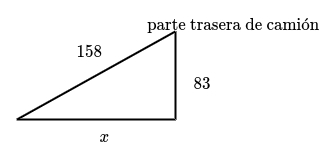
\includegraphics[width=0.5\textwidth]{../images/proverb_pitagoras_05.png}
    \end{center}
    \caption{}
    \label{fig:proverb_pitagoras_05}
\end{figure}
\textbf{¿Cuál es la distancia horizontal del extremo de la rampa a la parte trasera del camión?}
\textit{Redondea tu respuesta a la décima de centímetro más cercana.}